\documentclass[tikz,border=12pt]{standalone}
\usepackage[T1]{fontenc}
\usepackage{mathpazo}
\usepackage{amsmath,amssymb}
\usetikzlibrary{arrows.meta, positioning, calc}

\definecolor{stblue}{HTML}{7B97AD}
\definecolor{rwgold}{HTML}{B8995E}
\definecolor{sage}{HTML}{7A9A7E}
\definecolor{dkbrown}{HTML}{3D3530}
\definecolor{wmgray}{HTML}{7B7067}
\definecolor{cream}{HTML}{F9F6F0}
\definecolor{border}{HTML}{D4C9B8}
\definecolor{terracotta}{HTML}{C47A6A}

\begin{document}
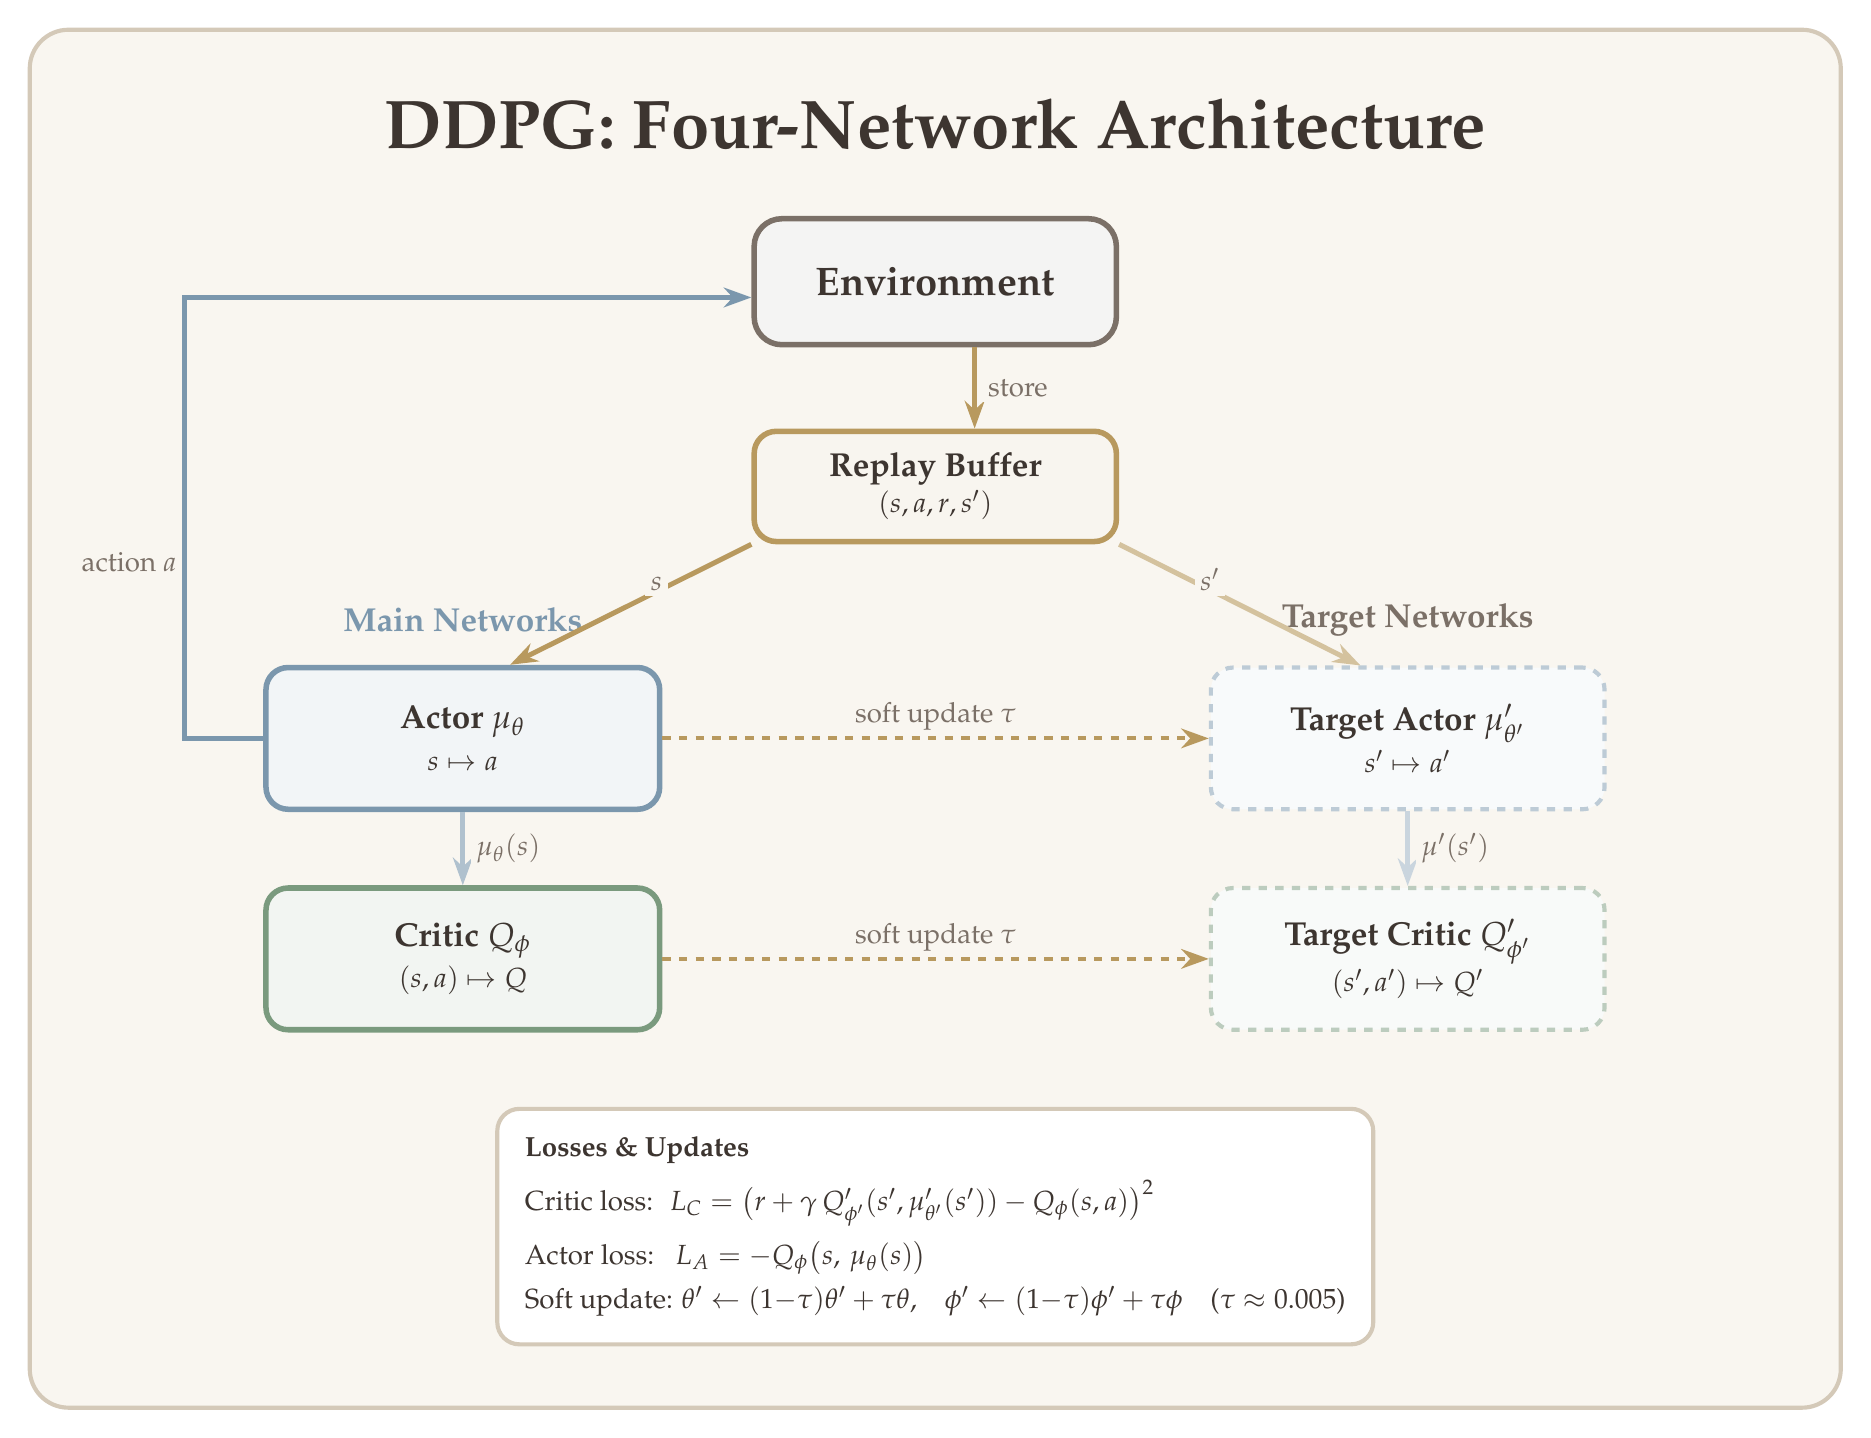
\begin{tikzpicture}[
  >={Stealth[length=3.5mm, width=2.5mm]},
  mainbox/.style={
    draw=#1, line width=2pt, fill=#1!10, rounded corners=8pt,
    minimum width=50mm, minimum height=18mm, font=\large, text=dkbrown,
    align=center, inner sep=6pt
  },
  tgtbox/.style={
    draw=#1!50, line width=1.5pt, fill=#1!5, rounded corners=8pt,
    minimum width=50mm, minimum height=18mm, font=\large, text=dkbrown,
    align=center, inner sep=6pt, dashed
  },
  arr/.style={->, line width=1.8pt, dkbrown},
  darr/.style={->, line width=1.5pt, dashed, rwgold},
  lbl/.style={font=\normalsize, text=wmgray, fill=cream, inner sep=2pt},
]

% Background
\fill[cream, rounded corners=14pt] (-1.5,-6.5) rectangle (21.5,11);
\draw[border, rounded corners=14pt, line width=1.5pt] (-1.5,-6.5) rectangle (21.5,11);

% Title
\node[font=\Huge\bfseries, text=dkbrown] at (10,9.8)
  {DDPG: Four-Network Architecture};

% =============================================
% Environment
% =============================================
\node[draw=wmgray, line width=2pt, fill=wmgray!8, rounded corners=10pt,
      minimum width=46mm, minimum height=16mm,
      font=\Large, text=dkbrown, align=center, inner sep=5pt]
  (env) at (10,7.8)
  {\textbf{Environment}};

% =============================================
% Replay Buffer
% =============================================
\node[draw=rwgold, line width=2pt, fill=rwgold!10, rounded corners=8pt,
      minimum width=46mm, minimum height=14mm,
      font=\large, text=dkbrown, align=center, inner sep=5pt]
  (buffer) at (10,5.2)
  {\textbf{Replay Buffer}\\[-1pt]
   {\normalsize $(s, a, r, s')$}};

% =============================================
% Section labels
% =============================================
\node[font=\large\bfseries, text=stblue] at (4, 3.5) {Main Networks};
\node[font=\large\bfseries, text=wmgray] at (16, 3.5) {Target Networks};

% =============================================
% Main Networks (left)
% =============================================
\node[mainbox=stblue] (actor) at (4, 2)
  {\textbf{Actor} $\mu_\theta$\\[1pt]
   {\normalsize $s \mapsto a$}};

\node[mainbox=sage] (critic) at (4, -0.8)
  {\textbf{Critic} $Q_\phi$\\[1pt]
   {\normalsize $(s, a) \mapsto Q$}};

% =============================================
% Target Networks (right, dashed)
% =============================================
\node[tgtbox=stblue] (actor-tgt) at (16, 2)
  {\textbf{Target Actor} $\mu'_{\theta'}$\\[1pt]
   {\normalsize $s' \mapsto a'$}};

\node[tgtbox=sage] (critic-tgt) at (16, -0.8)
  {\textbf{Target Critic} $Q'_{\phi'}$\\[1pt]
   {\normalsize $(s', a') \mapsto Q'$}};

% =============================================
% Arrows
% =============================================

% Env <-> Buffer
\draw[arr, rwgold] ([xshift=5mm]env.south) -- ([xshift=5mm]buffer.north)
  node[midway, right, lbl, xshift=2pt] {store};

% Actor -> Env (action): route left, up, then right to env
\draw[arr, stblue] (actor.west) -- ++(-1,0) |- ([yshift=-2mm]env.west)
  node[pos=0.2, left, lbl] {action $a$};

% Buffer -> Main networks (state s): diagonal
\draw[arr, rwgold] (buffer.south west) -- ([xshift=6mm]actor.north)
  node[pos=0.45, lbl, above right] {$s$};

% Buffer -> Target networks (next state s'): diagonal
\draw[arr, rwgold!60] (buffer.south east) -- ([xshift=-6mm]actor-tgt.north)
  node[pos=0.45, lbl, above left] {$s'$};

% Actor -> Critic (action for Q evaluation)
\draw[arr, stblue!60] (actor.south) -- (critic.north)
  node[midway, right, lbl, xshift=2pt] {$\mu_\theta(s)$};

% Target Actor -> Target Critic
\draw[arr, stblue!40] (actor-tgt.south) -- (critic-tgt.north)
  node[midway, right, lbl, xshift=2pt] {$\mu'(s')$};

% Soft update arrows (horizontal dashed)
\draw[darr] (actor.east) -- (actor-tgt.west)
  node[midway, above, lbl] {soft update $\tau$};
\draw[darr] (critic.east) -- (critic-tgt.west)
  node[midway, above, lbl] {soft update $\tau$};

% =============================================
% Loss box at bottom (informational)
% =============================================
\node[draw=border, line width=1.5pt, fill=white, rounded corners=8pt,
      font=\normalsize, text=dkbrown, align=left, inner sep=10pt]
  at (10,-4.2)
  {\textbf{Losses \& Updates}\\[5pt]
   Critic loss:\; $L_C = \bigl(r + \gamma\, Q'_{\phi'}(s', \mu'_{\theta'}(s')) - Q_\phi(s, a)\bigr)^2$\\[4pt]
   Actor loss:\;\, $L_A = -Q_\phi\bigl(s,\, \mu_\theta(s)\bigr)$\\[4pt]
   Soft update: $\theta' \leftarrow (1{-}\tau)\theta' + \tau\theta$,\quad
   $\phi' \leftarrow (1{-}\tau)\phi' + \tau\phi$\quad ($\tau \approx 0.005$)};

\end{tikzpicture}
\end{document}
